\documentclass[runningheads]{comsis2}

%% Necessary definitions for the running heads
\def\journalissue{Computer Science and Information Systems 00(0):0000--0000}
\def\paperidnum{https://doi.org/10.2298/CSIS123456789X}
\setcounter{page}{1}

%% Use this to show line numbers (and remove only in the final camera-ready version)
\usepackage[pagewise]{lineno}
\linenumbers
\usepackage{hyperref}
\usepackage{verbatim}
\usepackage{graphicx}
\usepackage{amsmath}
\usepackage[normalem]{ulem}


%%%%% NEW PACKAGES 
\usepackage{graphicx}
\usepackage{color, colortbl}
\graphicspath{ {./figures/} }

\newcommand*{\Comb}[2]{{}C^{#1}_{#2}}%
%%%%%%%

\title{Logical dependencies: extraction from the versioning system and usage in key classes detection}

%% Use this if the title is too long for the running heads
\titlerunning{Logical dependencies in practice}

\author{Adelina Diana Stana\inst{1} \and Ioana Şora\inst{1}}

%% Use this the list of authors is too long for the running heads
%\authorrunning{First Author et al.}

\institute{
 Politehnica University, Piaţa Victoriei Nr. 2, ; 300006 Timişoara, jud. Timiş, România\\
  \email{stana.adelina.diana@gmail.com; ioana.sora@cs.upt.ro}
}

\begin{document}

\maketitle

\begin{abstract}
The version control system of every software product can provide important information about how the system is connected.
In this study, we first propose a language-independent method to collect and filter dependencies from the version control, and second, we use the results obtained in the first step to identify key classes from three software systems. To identify the key classes, we are using the dependencies extracted from the version control system together with dependencies from the source code, and also separate. Based on the results obtained we can say that compared with the results obtained by using only dependencies extracted from code, the mix between both types of dependencies provides small improvements. And, by using only dependencies from the version control system, we obtained results that did not surpass the results previously mentioned, but are still acceptable.
We still consider this an important result because this might open an important opportunity for software systems that use dynamically typed languages such as JavaScript, Objective-C, Python, and Ruby, or systems that use multiple languages. These types of systems, for which the code dependencies are harder to obtain, can use the dependencies extracted from the version control to gain better knowledge about the system.
  
\vspace{6pt}\textbf{Keywords:} logical dependencies; logical coupling; mining software repositories; versioning system; key classes; co-changing entities; software evolution.
\end{abstract}


\section{Introduction}

The version control (also known as source control) system that tracks changes in source code during software development can provide useful information about the system's details. 
The usage of information extracted from the version control system is not new. Previous works have used version control information to detect design issues \cite{Zimmermann:2004:MVH:998675.999460}, predict fault incidence among modules \cite{Predictingfaultincidence}, \cite{Cataldo2009SoftwareDW}, reconstructing software development methods \cite{article_comsis} or guide software changes \cite{4815274}, \cite{DBLP:journals/ese/AjienkaCC18}.
In software engineering literature, concepts like evolutionary coupling, evolutionary dependencies, logical dependencies, or logical coupling refer to the same sort of relationship among software entities. That relationship is extracted from the version control system and can mean that the entities from the source code files change together, evolve together, and might depend on one another. Studies show that dependency relationships found in the source code overlap only in a small percentage with dependency relationships found in the version control system, and suggest that these two types of relationships can be used together \cite{Oliva:2011:ISL:2067853.2068086}, \cite{DBLP:journals/jss/AjienkaC17}. But, in practice, dependencies extracted from the version management system are rarely used because of the size of the information extracted \cite{Shtern:2012:CMS:2332427.2332428}. A relatively small source code repository with roundabout one thousand commits can lead to millions of connections. 
In this paper, by applying a set of filters with different thresholds to the information extracted, we intend to speed up the processing time, reduce the size of connections extracted from the version control and increase the confidence that the connections obtained might be related.
To validate the results obtained, and to see if the filtering methods had or had not a favorable effect on the final result, we want to identify the key classes of different systems. The identification of key classes has been previously performed by using structural dependencies, so
we intend to use the results obtained together with structural dependencies, and also separate, and see how the final results fluctuate.

In this work we perform our analysis on three open
source projects: Ant, Tomcat Catalina, and Hibernate. And we answer the following research questions:

\textbf{RQ1: Will logical dependencies combined with structural dependencies enhance results previously obtained?}
Since previous researches and our studies show that logical dependencies overlap only in a small percentage with structural dependencies, we intend to combine both types of dependencies and provide them as input for key classes identification tools.

\textbf{RQ2: Can logical dependencies provide good results if used instead of structural dependencies?}
In this research question, we want to focus more on the use of logical dependencies as stand-alone dependencies. Even though logical dependencies are not the same as structural dependencies, they can provide enough information about the system to be successfully used as input for tools like key classes detection tools. 

\textbf{RQ3: Does the connection strength filter has a favorable impact on the results obtained?}
In this paper, we use a new type of filter: the connection strength filter. This filter, together with the commit size filter, will be used to filter co-changes into logical dependencies. Now, the question is if this new filter will indeed do what we expect and provide better results.

\textbf{Paper structure.} The paper is organized as follows: Section \ref{ld_def} introduces the concepts of logical dependencies and the methods of obtaining them. Section \ref{sec:baseline_approach} introduces the concept of key classes and the metrics used for results evaluation. The new approach of using logical dependencies to detect key classes can be found in section \ref{sec:keycalss_identification}. Section \ref{sec:current_measurements} defines the data set used and presents the new results obtained with the data set. In section \ref{sec:threats} we present the threats to the validity of the results presented in this paper. And finally, section \ref{sec:conclusion} discusses the conclusions based on the results obtained. 




\section{The concept of logical dependencies}
\label{ld_def}
This section presents the definition of logical dependencies, previous works involving logical dependencies, and our contribution to this topic. In subsection \ref{definition_ld}, we define what logical dependencies are and the previous research involving them. In subsection \ref{current_approach}, we present our approach for identifying logical dependencies and the work we have done around this subject. Related to subsection \ref{current_approach}, sections \ref{commit_filter}, and \ref{strength_filter} present more details about the filtering techniques we used to identify logical dependencies.

\subsection{Definition and previous related research}
\label{definition_ld}
The concept of logical coupling (dependency) was first introduced by Gall et al. \cite{Gall:1998:DLC:850947.853338}. They defined the logical dependency between two software entities (classes, modules, interfaces, etc.) as the fact that the entities repeatedly change together during the historical evolution of a software system.
Since then, logical dependencies have been used in multiple areas of software engineering, most commonly in fault and change prediction.  
Besides the studies on how logical dependencies can help gain knowledge about software systems, some studies also focused on the interplay between logical and structural dependencies. Ajienka et al. and Olivia et al. studied the interplay between structural and logical dependencies, and they concluded that, in most cases, structural dependencies do not lead to logical dependencies \cite{Oliva:2011:ISL:2067853.2068086}, \cite{DBLP:conf/issre/OlivaG15}, \cite{DBLP:journals/jss/AjienkaC17}. The above affirmation is also supported by Lanza et al., who consider that logical dependencies are important because they can reveal dependencies that are not visible via code analysis \cite{inproceedings_radar_evolution}.



In previous research, the \textit{support} and \textit{confidence} metrics were used to measure the strength of a logical dependency. 
The logical dependencies are commonly represented as directed association rules \cite{DBLP:conf/issre/OlivaG15}, \cite{DBLP:journals/jss/AjienkaC17}, \cite{Zimmermann:2004:MVH:998675.999460}. The association rule between A and B ( $A \rightarrow B$) means that changes in entity A cause changes in entity B, where A is the antecedent, and B is the consequent of the rule. 
The support metric counts the number of commits in which both entities of an association rule change together. The confidence metric is the ratio between the support metric and the total number of commits in which the antecedent of the rule was involved. 

By applying different thresholds to the metrics presented above, the logical dependencies to further use were selected.


\subsection{Our approach for logical dependencies identification}
\label{current_approach}

To avoid confusion, we call \textit{co-changing pairs} all the association rules of one system. The association rules are formed between two software entities that update together in the same commit.
For example, a commit that contains seven entities will generate 21 co-changing pairs ($\Comb{n}{k}=\frac{n!}{k!(n-k)!} = \frac{7!}{2!(5)!} = 21$).


The \textit{logical dependencies} are the association rules whose metrics fulfill certain conditions. So, the logical dependencies are a subset of the co-changing pairs. 

The conditions that need to be met by a co-changing pair to be considered a logical dependency are called \textit{filters}. Like in other research regarding logical dependencies, our filters are thresholds applied to the metrics of association rules. 

Previously, we tried to filter logical dependencies from co-changing pairs by applying filters like the occurrence filter and commit size filter \cite{saci19}, \cite{enase19}. 
The commit size filter, presented in more detail in section \ref{commit_filter}, and used by other authors \cite{DBLP:journals/jss/AjienkaC17}, proved to be helpful, and it will be also used for this paper. 
But we cannot say the same for the occurrence filter. The filter consisted of different thresholds applied to the support metric and proved to not work well for systems with few commits.

Currently, we aim to refine the filtering method with a new filter applicable to all sorts of commit history sizes. This new filter, presented in section \ref{strength_filter}, will be used together with the commit size filter to filter logical dependencies from co-changing pairs. The entire process of extracting co-changing pairs from the versioning system, filtering them to obtain logical dependencies, and exporting the results, is done with a tool written in Python. The workflow is presented in figure \ref{fig:workflow_key}.

\begin{figure}
\centering
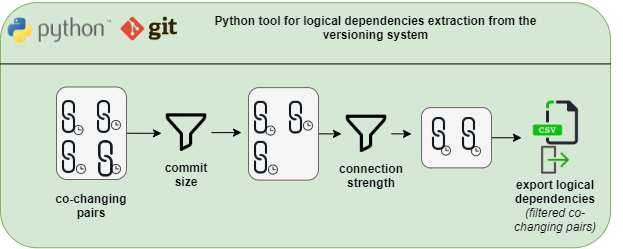
\includegraphics[scale=0.6]{ld_workflow.png}
\caption{Workflow for logical dependencies extraction.}
\label{fig:workflow_key}
\centering
\end{figure}

\subsection{Logical dependencies filtering: The commit size filter}
\label{commit_filter}

The commit size filter filters out all co-changing pairs from commits with more than 10 files changed. We consider that commits with more than 10 files changed tend to be code unrelated; we studied the commit size trend from serval git open-source repositories, and we concluded that most of the commits contain less than 10 files. On average, only 10\% of the total commits have more than 10 files changed. 

This filter will also prevent the volume of data processed from going out of proportion. In some of the repositories studied, we found commits with more than 1000 files; these commits could generate over half a million co-changing pairs if the commit size filter is not applied \cite{enase19}, \cite{saci19}. 



\subsection{Logical dependencies filtering: The connection strength filter}
\label{strength_filter}


The connection strength filter is new for our research regarding logical dependencies identification, and it is based on our experience with the occurrence filter.
An important conclusion drawn from the results obtained with the occurrence filter is that setting a hard threshold for a filter is not always a good idea. A certain threshold can work well with a medium/large-sized system, but when applied to a small-sized system, it can reduce the co-changes filtered to 0. To avoid this kind of situation, we evaluated a filter that considers the system's specifications. 


As we previously mentioned, a filter has two components: the metrics computed for each co-changing pair (association rule) and the threshold values. The connection strength metric derives from the support and the confidence metrics.

For an association rule (co-changing pair) formed from the antecedent A and consequent B ($A \rightarrow B$), 
the support count is the total number of commits in which both entities are involved,


\begin{equation}
support (A \rightarrow B) = freq_{total\ commits} {(A \cup B)}
\end{equation}

and the confidence is the ratio between the support and the frequency of the antecedent of the rule.

\begin{equation}
confidence (A \rightarrow B) =\frac{support (A \rightarrow B) }{freq_{total\ commits}(A)}
\end{equation}


The only problem with the confidence metric, as it is defined above, is that it does not include the big picture of the system.
The best value for the confidence metric is 1, meaning that in all commits in which entity A is present, entity B is also there. If, for example, we have a co-changing pair $A \rightarrow B$, and A updates only once in the entire history, and in that time, updates together with B, then the confidence metric associated with the co-changing pair will be 1 (the best value possible). That is not a fair value compared with other scenarios. For example, we can have the co-changing pair $A \rightarrow B$, and A updates 100 in the entire history from which 80 times updates together with B, leading to a confidence value of 0.8.
Even though in the second scenario we have a confidence value smaller than in the first scenario, the second scenario could lead to a more trustworthy connection.

Figures \ref{fig:strength_overview_ant} and \ref{fig:strength_overview_hibernate}  intend to offer the big picture of two systems, one small-sized (Ant) and one medium-sized (Hibernate). In both figures, the dots represent the maximum number of updates of one entity with another, and the blue line represents the average occurrence value of the system.
It can be observed that both systems have multiple entities that update only once (the dark line at the bottom), meaning that we might have many confidence values of 1 (the highest value possible) for entities that update only once together.

\begin{figure}
\centering
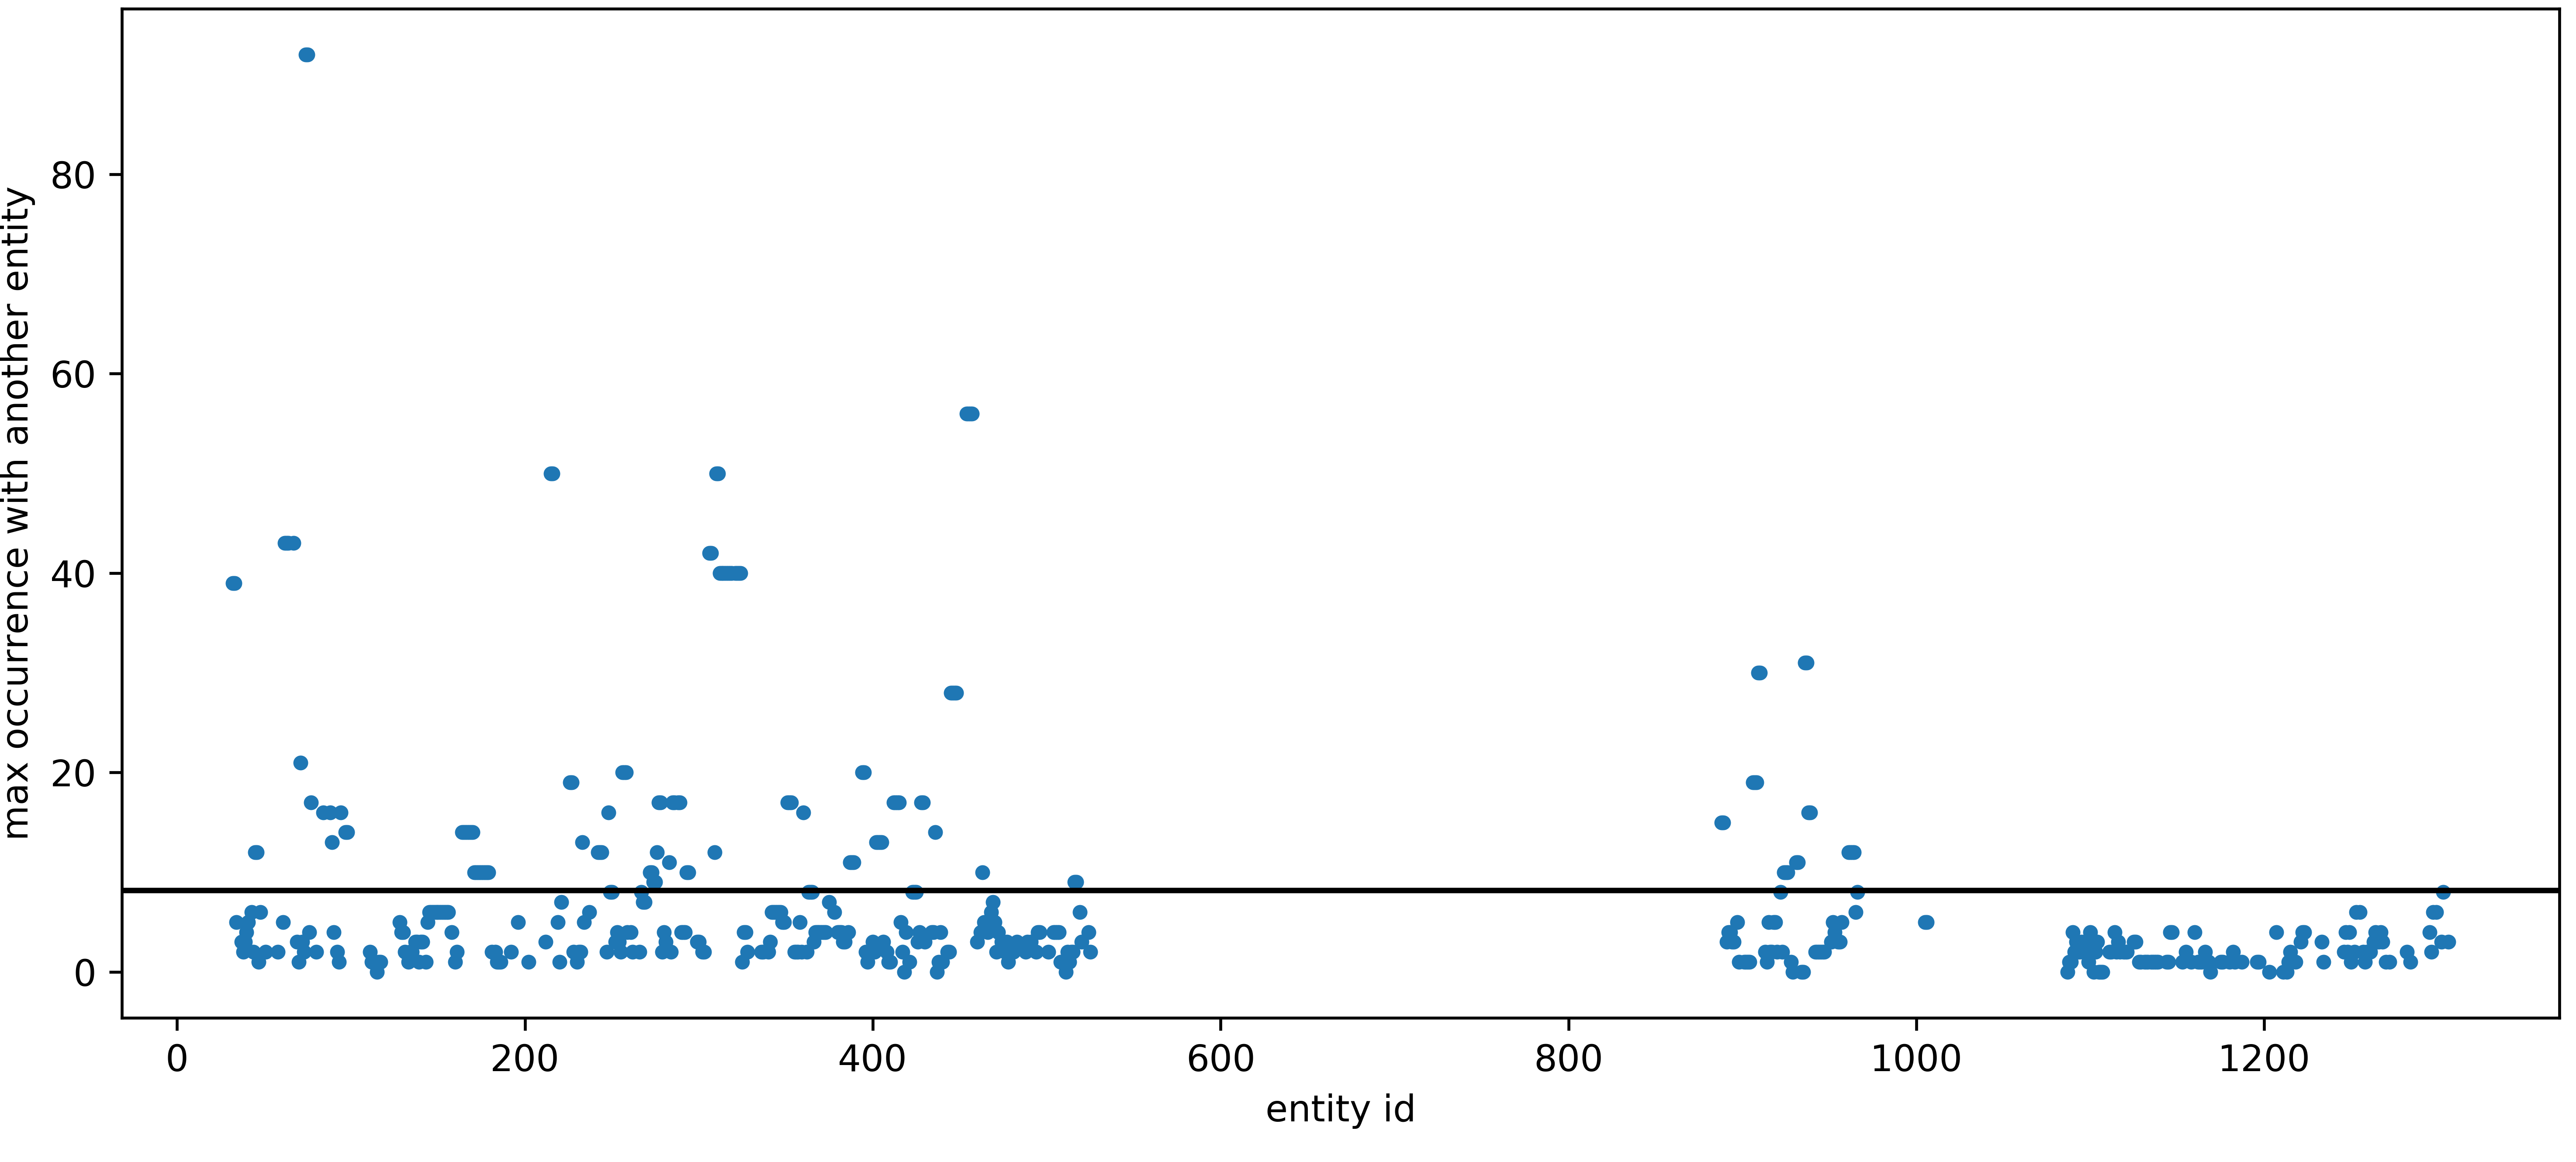
\includegraphics[scale=0.63]{fig_ant_maxOcc.png}
\caption{Overview of the number of occurrences in Ant. }
\label{fig:strength_overview_ant}
\centering
\end{figure}

\begin{figure}
\centering
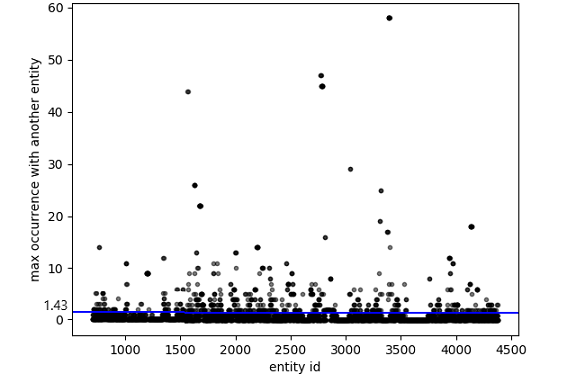
\includegraphics[scale=0.63]{fig_hibernate_maxOcc.png}
\caption{Overview of the number of occurrences in Hibernate. }
\label{fig:strength_overview_hibernate}
\centering
\end{figure}

To take into account the big picture of the system, we defined a new metric for a co-changing pair (association rule), called the \textit{connection strength metric}. 

The connection strength metric is computing the same ratio as the confidence metric, a.k.a the ratio between the support metric and the frequency of the antecedent. And additionally, it multiplies it with a system factor and with 100. 
The \textit{system factor} calculates the ratio between the support metric and the mean value for updates. The \textit{system mean} is the mean value of all the support values for all the association rules from the system. 
We multiply with 100 because we want to scale the metric's values to structural dependencies metric's values that have, in most cases, supraunitary values. And we want both metrics to be comparable. The values obtained are clipped between 0 and 100, where 100 is the best value and 0 is the worst.

\begin{equation}
 system factor for (A \rightarrow B) =\frac{support (A \rightarrow B) }{system\ mean}
\end{equation}

\begin{equation}
 strength (A \rightarrow B) =\frac{support (A \rightarrow B) * 100}{freq_{total\ commits}(A)} * system\ factor
\end{equation}

By using the strength metric, if we consider again the two scenarios presented above, and a system mean value of 10, we will have the following values: for the scenario in which the entities A and B update only once, and in that one update, they update together, the strength metric value is 10. For the scenario in which entity A updates 100 times in the entire history from which 80 times updates together with B, the strength metric value is 100.  




Since the values can vary from 0 to 100, the filter threshold values begin at 10 and are repeatedly incremented by 10, until 100. We do not settle for one value because we want to see how the threshold values affect the number of remaining co-changing pairs and the output of their usage.

In figure \ref{fig:strength_overview} we plotted for two systems (one small-sized and one medium-sized) the number of structural dependencies, co-changing pairs before filtering, and co-changing pairs after filtering. With the connection strength filter, the small-sized system didn't lose all the co-changing pairs once with the filtering.
We compare the number of remaining co-changing pairs with the number of structural dependencies because, according to surveys \cite{Shtern:2012:CMS:2332427.2332428}, \cite{sar}, the main reason why logical dependencies (filtered co-changes) are not used together with structural dependencies is their size. So, it is essential to get an overview of the comparison between the number of co-changing pairs and the number of structural dependencies at each filtering step.

We call the co-changing pairs that remain after filtering, logical dependencies. 
After this step, we will use the logical dependencies obtained with different threshold values and see which threshold value performs the best. Up until now, we only looked at the size of the resulting logical dependencies and decided if a filter and its threshold are good or not. Now, we can also look at the results obtained by using the logical dependencies and decide.

\begin{figure}
\centering
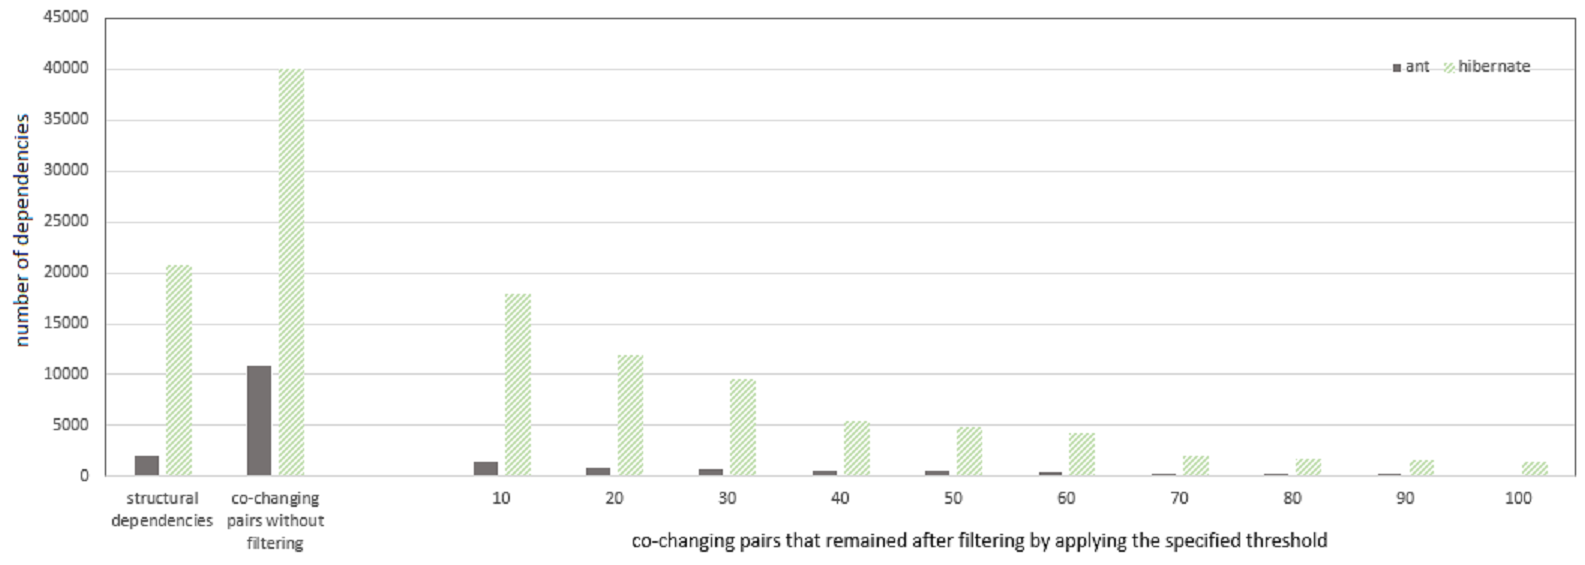
\includegraphics[width=\textwidth]{strength_overview.PNG}
\caption{Overview of the impact of connection strength filtering on the number of co-changing pairs. }
\label{fig:strength_overview}
\centering
\end{figure}



\section{The concept of key classes}
\label{sec:baseline_approach}

This section presents the key classes definition, previous research regarding key classes identification, and metrics used to evaluate the results obtained.
In section \ref{sec:keyclass_definition}, we present a summary of previous researchers and their approaches to key classes identification. Section \ref{sec:baseline_approach_sub} focuses on one previous research that we consider as our baseline research in key classes identification. With the results of the baseline research, we will compare our results. 
In section \ref{sec:evalmetrics}, we present the metrics used in previous research to evaluate the results obtained. 


\subsection{Definition and previous research}
\label{sec:keyclass_definition}

Zaidman et al. \cite{ZaidmanJurnal} was the first to introduce the concept of key classes and it refers to classes that can be found in documents written to provide an architectural overview of the system or an introduction to the system structure.
Tahvildari and Kontogiannis have a more detailed definition regarding the key classes concept: “Usually, the most important concepts of a system are implemented by very few key classes which can be characterized by the specific properties. These classes, which we refer to as key classes, manage many other classes or use them in order to implement their functionality. The key classes are tightly coupled with other parts of the system. Additionally, they tend to be rather complex, since they implement much of the legacy system’s functionality” \cite{Tahvildari2004ImprovingDQ}.


The key class identification can be done by using different algorithms with different inputs. In the research of Osman et al., the key class identification is made by using a machine learning algorithm and class diagrams as input for the algorithm \cite{6676885}. Thung et al. built on top of Osman et al.’s approach and added network metrics and optimistic classification to detect key classes \cite{rocclasification}.

Zaidman et al. used a web mining algorithm and dynamic analysis of the source code to identify the key classes \cite{ZaidmanJurnal}.

\subsection{Baseline approach}
\label{sec:baseline_approach_sub}
We use the research of I. Şora et al. \cite{Finding-key-classes} as a baseline for our research involving the usage of logical dependencies to find key classes. 

Şora et al. used the static analysis of the source code, a page ranking algorithm and other class attributes to find key classes \cite{PagerankENASE}, \cite{enase15}, \cite{SoraSpringer}, \cite{PagerankSACI},\cite{Finding-key-classes}.
The page ranking algorithm is a customization of PageRank, the algorithm used to rank web pages \cite{ilprints422}, and it works based on a recommendation system. If one node has a connection with another node, then it recommends the second node. In previous research, connections are established based on structural dependencies extracted from static code analysis. If A has a structural dependency with B, then A recommends B, and also B recommends A.

The ranking algorithm ranks all the classes from the source code of the system, according to their importance. To identify the important classes from the rest, a threshold for the top classes from the top of the ranking is set. We call this TOP threshold, and its value can range from 1 to the total number of classes found in the system. 

\subsection{Metrics for results evaluation}
\label{sec:evalmetrics}
To evaluate the quality of the key classes ranking algorithm and solution produced, the key classes found by the algorithm are compared with a reference solution. The reference solution is extracted from the developer documentation. The classes mentioned in the documentation are considered key classes and form the reference solution (ground truth) used for validation \cite{7551990}.

For the comparison between both solutions, a classification model is used. The quality of the solution produced is evaluated by using the Receiver Operating Characteristic Area Under Curve (ROC-AUC) metric, a metric that evaluates the performance of a classification model.


The ROC graph is a two-dimensional graph that has on the X-axis plotted the false positive rate and on the Y-axis the true positive rate. By plotting the true positive rate and the false positive rate at thresholds that vary between a minimum and a maximum possible value, we obtain the ROC curve. The area under the ROC curve is called Area Under the Curve (AUC).

The true positive rate of a classifier is calculated as the division between the number of true positive results identified, and all the positive results identified:

\begin{equation}
 True\ positive\ rate (TPR) = \frac{TP}{TP+FN}
\end{equation}
The false positive rate of a classifier is calculated as the division between the number of false positive results identified, and all the negative results identified:

\begin{equation}
 False\ positive\ rate (FPR) = \frac{FP}{FP+TN}
\end{equation}

The True Positives (TP) are the classes found in the reference solution and also in the top TOP ranked classes. False Positives (FP) are the classes that are not in the reference solution, but are in the TOP ranked classes.
True Negatives (TN) are classes that are found neither in the reference solution nor in the TOP ranked classes. False Negatives (FN) are classes that are found in the reference solution, but are not found in the TOP ranked classes.

In related research, the ROC-AUC metric has been used to evaluate the results for finding key classes of software systems.
For a classifier to be considered good, its ROC-AUC metric value should be as close to 1 as possible.
When the value is 1, then the classifier is considered to be perfect. A metric value between 0.8 and 0.9 means that the classifier is excellent. Between 0.8 and 0.7 means acceptable results, and between 0.7 and 0.5 means poor results \cite{ROC_METRIC_VALS}. 


\section{Key classes identification using logical dependencies}
\label{sec:keycalss_identification}
This section presents our approach for key classes identification by using logical dependencies. 
In section \ref{sec:current_approach}, we describe the experimental setup and how we intend to integrate logical dependencies with the baseline approach. 
Section \ref{sec:plan} presents our investigation plan and how this plan can respond to the research questions we enunciated at the beginning of this paper.

\subsection{Current approach}
\label{sec:current_approach}
The baseline approach uses a tool that takes as an input the source code of the system and applies ranking strategies to rank the classes according to their importance. We modified the tool used by the baseline approach to take also the logical dependencies as input; the rest of the workflow is the same as in the baseline approach (figure \ref{fig:baseline_approach}).

\begin{figure}
\centering
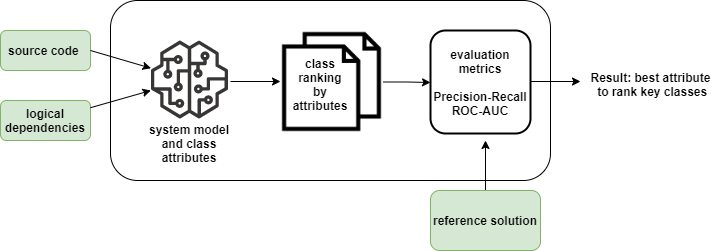
\includegraphics[width=\textwidth]{current_approach.PNG}
\caption{Overview of the current approach.}
\label{fig:baseline_approach}
\centering
\end{figure}
Below are some of the class metrics used in the baseline approach and in our current research to rank the classes according to their importance. 

The class metrics used can be separated into two categories: class connection metrics and class PageRank values.
The class connection metrics are CONN-TOTAL-W, which is the total weight of all connections of the class, and CONN-TOTAL, the total number of distinct classes that a class uses or is using the class \cite{Finding-key-classes}.

Previous research used PageRank values computed on both directed and undirected, weighted and unweighted graphs. In the current research, we use the PR, which is the PageRank value computed on the directed and unweighted graph, the PR-U, which is the value computed on the undirected and unweighted graph, and the PR-U2-W, the value computed on the weighted graph with back-recommendations \cite{PagerankENASE}, \cite{enase15}, \cite{Finding-key-classes}, \cite{PagerankSACI}.


\subsection{Experimental plan}
\label{sec:plan}

Our study aims to check whether logical dependencies can be usable. Previous research focused on filtering the co-changes extracted from the versioning system and studying how filtering affects their size or how they overlap with structural dependencies. We intend to use the resulting information after co-changes filtering (the logical dependencies) in a tool that usually receives structural dependencies as input.

Our research questions are the following: \textbf{RQ1:} \textit{Will logical dependencies combined with structural dependencies enhance results previously obtained?} \textbf{RQ2:} \textit{Can logical dependencies provide good results if used instead of structural dependencies?} \textbf{RQ3:} \textit{ Does the connection strength filter has a favorable impact on the results obtained?}

To answer the research questions, we defined the following experimental plan: 
We will use the tool mentioned in the above section. Previously the tool had as input the structural dependencies of the system and the reference solution, and the output was the ROC-AUC score. The closer the ROC-AUC score is to 1, the better the results.  
With the slightly modified version of the tool, we are able to receive as input also logical dependencies.


For \textbf {RQ1}, we will give as input to the tool the structural and the logical dependencies, and we will compare the ROC-AUC scores obtained with the results obtained by using only structural dependencies.


\noindent\fbox{%
    \parbox{\textwidth}{%
      \textit{Hypothesis:} Key classes detection is better when we provide both types of dependencies as input to the tool. The output has a higher ROC-AUC score than the base approach.
    }%
}
\medskip

Our findings for this research question can be found in section \ref{sec:measure_ld_sd}.


For \textbf {RQ2}, we will give as input to the tool only logical dependencies, and we will compare the ROC-AUC scores obtained with the results obtained by using only structural dependencies, and by using structural and logical dependencies combined.
We do not expect that the results will be better compared to the results previously obtained, but we expect results that have a ROC-AUC score close to those values. That would mean that logical dependencies can provide enough information to detect most of the key classes of the system.

\medskip

\noindent\fbox{%
    \parbox{\textwidth}{%
      \textit{Hypothesis:} The output has a ROC-AUC score between 0.7 and 1. 
    }%
}

\medskip

Our findings for this research question can be found in section \ref{sec:measure_ld}.

For \textbf {RQ3}, we will generate two sets of logical dependencies. One set will be generated with the connection strength filter and one with the confidence filter. We will then use each set in two different scenarios: one when we only use logical dependencies to detect key classes and one when we use logical and structural dependencies for detection. Finally, we will compare the results obtained. We expect that the connection strength filter will generate better results. 

\medskip

\noindent\fbox{%
    \parbox{\textwidth}{%
      \textit{Hypothesis:} The results obtained by using the connection strength filter are better than the ones obtained with the confidence filter. 
    }%
}

\medskip
Our findings for this research question can be found in section \ref{sec:measure_metrics}.

\section{Experimental results using logical dependencies}
\label{sec:current_measurements}


As presented in section \ref{sec:baseline_approach}, the key class detection was previously done only by using the structural dependencies of the system. 
In this section, we use the same tool used in the baseline approach presented in section \ref{sec:baseline_approach}, and we add a new input to it, the logical dependencies. 

In subsection \ref{sec:dataset}, we present the data set used to generate new results and, in subsection \ref{sec:measure_baseline}, we present the previously obtained results. Subsection \ref{sec:measure_ld_sd} presents the conclusions and results obtained by using logical and structural dependencies together, and subsection \ref{sec:measure_ld} presents the conclusions and results obtained by using only logical dependencies. Subsection \ref{sec:measure_metrics} presents a comparison between results obtained with the confidence metric versus results obtained with the strength metric. And finally, subsection \ref{sec:compare_others} presents a comparison between the results obtained in the current paper and the results of other researchers.


\subsection{Data set used}
\label{sec:dataset}


The research of I. Sora et al. take into consideration structural dependencies that were extracted using static analysis techniques and were performed on the object-oriented systems presented in table \ref{tab:gitfoundsystems} \cite{Finding-key-classes}.

The requirements for a system to qualify as suited for investigations using logical dependencies are: has to be version controlled by Git, has to have releases for different code versions (previous research was done only on specific versions), and also has to have a significant number of commits. 
From the total of 14 object-oriented systems listed in the baseline \cite{Finding-key-classes}, 13 of them have repositories in git \ref{tab:gitfoundsystems}, and from the found repositories, only 6 repositories have the same release tag as the specified version in previous research.
The commit number found on the remaining 6 repositories varies from 19108 commits for Tomcat Catalina to 149 commits for JHotDraw. In order to have more accurate results, we need a significant number of commits (more than 5000 commits), so we concluded to use only 3 systems from the initial candidates for key classes detection using logical dependencies:  Ant, Hibernate, and Tomcat Catalina.  

\begin{table}
\renewcommand{\arraystretch}{1}
\caption{Systems and versions of the systems found in Git. }
\label{tab:gitfoundsystems}
\centering
\scalebox{0.9}{
\begin{tabular}{lllll}
\hline
ID	&	System	&	Version	&	Release Tag name	&	Commits number	\\
\hline
Sl	&	Apache Ant	&	1.6.1	&	rel/1.6.1	&	6713	\\
S2	&	Argo UML	&	0.9.5	&	not found	&	0	\\
S3	&	GWT Portlets	&	0.9.5 beta	&	not found	&	0	\\
S4	&	Hibernate 	&	5.2.12	&	5.2.12	&	6733	\\
S5	&	javaclient	&	2.0.0	&	not found	&	0	\\
S6	&	jEdit	&	5.1.0	&	not found	&	0	\\
S7	&	JGAP	&	3.6.3	&	not found	&	0	\\
S8	&	JHotDraw	&	6.0b.1	&	not found	&	149	\\
S9	&	JMeter	&	2.0.1	&	v2\_1\_1	&	2506	\\
S10	&	Log4j	&	2.10.0	&	v1\_2\_10-recalled	&	634	\\
S11	&	Mars	&	3.06.0	&	not found	&	0	\\
S12	&	Maze	&	1.0.0	&	not found	&	0	\\
S13	&	Neuroph	&	2.2.0	&	not found	&	0	\\
S14	&	Tomcat Catalina	&	9.0.4	&	9.0.4	&	19108	\\
S15	&	Wro4J	&	1.6.3	&	v1.6.3	&	2871	\\
\hline
\end{tabular}
}
\end{table}

\subsection{Measurements using only the baseline approach}
\label{sec:measure_baseline}

In table \ref{tab:previousresults} are presented the ROC-AUC values for different attributes computed for the systems Ant, Tomcat Catalina, and Hibernate by using the baseline approach. We compare these values with the new values obtained by using also logical dependencies in key class detection.

\begin{table}
\renewcommand{\arraystretch}{1}
\caption{ROC-AUC metric values extracted. }
\label{tab:previousresults}
\centering
\scalebox{0.9}{
\begin{tabular}{|c|ccc|}
\hline
Metrics &	Ant	&	Tomcat Catalina	&	Hibernate	\\
\hline

PR\_U2\_W	&	0.95823	&	0.92341	&	0.95823	\\
PR	&	0.94944	&	0.92670	&	0.94944	\\
PR\_U	&	0.95060	&	0.93220	&	0.95060	\\
CONN\_TOTAL\_W	&	0.94437	&	0.92595	&	0.94437	\\
CONN\_TOTAL	&	0.94630	&	0.93903	&	0.94630	\\
\hline
\end{tabular}
}
\end{table}


\subsection{Measurements using combined structural and logical dependencies}
\label{sec:measure_ld_sd}

The tool used in the baseline approach runs a graph-ranking algorithm on a graph that contains all the structural dependencies extracted from static source code analysis.
Each edge in the graph represents a dependency. The entities that form a structural dependency are represented as vertices in the graph. 
As mentioned in section \ref{sec:baseline_approach}, we modified the tool to take structural and logical dependencies as input.
For this subsection's measurements, we add the logical dependencies in the graph that contains all structural dependencies. Since it is a weighted graph, if a structural dependency is also a logical dependency, then the final weight of the connection is the sum of the weight computed for the structural dependency and the connection strength metric associated with the logical dependency.

In tables \ref{tab:measurementscombined:ant}, \ref{tab:measurementscombined:tomcat}, and \ref{tab:measurementscombined:hibernate}, on each line, we have the computed the key class metric generated with logical dependencies extracted with the connection strength threshold that is specified in the colums header.

We started with logical dependencies that have a connection strength metric greater than 10, then we repeatedly increased the value by 10 until we reached 100. The last column of the table contains the results previously obtained by the tool by only using structural dependencies (the results presented in section \ref{sec:measure_baseline}).

So, to answer \textit{RQ1: Will logical dependencies combined with structural dependencies enhance results previously obtained?}:

The results obtained by combining structural and logical dependencies are close to the previously registered values but, in most cases, do not surpass them. Underlined are the values that are better than the previously registered values. We can observe that for all 3 systems, the best values obtained are for connection strength between 40-70.

\begin{table}[!h]
\setlength\tabcolsep{3.5pt}
\caption{Measurements for Ant using structural and logical dependencies combined}
\label{tab:measurementscombined:ant}
\centering
\scalebox{0.9}{
\begin{tabular}{|c|cccccccccc|c|}
\hline
Metrics &	$\geq10$	&	$\geq20$		&	$\geq30$		&	$\geq40$		&	$\geq50$		&	$\geq60$		&	$\geq70$		&	$\geq80$		&	$\geq90$		&	$\geq100$		&	Baseline \\
\hline
PR\_U2\_W	&	0.877	&	0.880	&	0.883	&	0.888	&	0.884	&	0.880	&	0.901	&	0.924	&	0.900	&	0.891	&	0.929	\\
PR	&	\underline{0.955}	&	\underline{0.932}	&	\underline{0.936}	&	\underline{0.936}	&	\underline{0.880}	&	\underline{0.884}	&	\underline{0.887}	&	\underline{0.889}	&	\underline{0.888}	&	\underline{0.890}	&	0.855	\\
PR\_U	&	0.933	&	\underline{0.937}	&	\underline{0.936}	&	\underline{0.939}	&	\underline{0.940}	&	\underline{0.939}	&	\underline{0.941}	&	\underline{0.943}	&	\underline{0.942}	&	\underline{0.940}	&	0.933	\\
CON\_T\_W	&	0.841	&	0.839	&	0.836	&	0.838	&	0.835	&	0.849	&	0.859	&	0.872	&	0.870	&	0.874	&	0.934	\\
CON\_T	&	0.920	&	0.919	&	0.921	&	0.923	&	0.923	&	0.932	&	0.934	&	0.939	&	0.937	&	0.937	&	0.942	\\
\hline
\end{tabular}
}
\end{table}


\begin{table}[!h]
\setlength\tabcolsep{3.5pt}
\caption{Measurements for Tomcat Catalina using structural and logical dependencies combined}
\label{tab:measurementscombined:tomcat}
\centering
\scalebox{0.9}{
\begin{tabular}{|c|cccccccccc|c|}
\hline
Metrics &	$\geq10$	&	$\geq20$		&	$\geq30$		&	$\geq40$		&	$\geq50$		&	$\geq60$		&	$\geq70$		&	$\geq80$		&	$\geq90$		&	$\geq100$		&	Baseline \\
\hline
PR\_U2\_W	&	0.862	&	0.883	&	0.898	&	0.901	&	0.907	&	0.909	&	0.910	&	0.916	&	0.918	&	0.918	&	0.923	\\
PR	&	0.879	&	0.885	&	0.888	&	0.882	&	0.869	&	0.869	&	0.863	&	0.863	&	0.863	&	0.863	&	0.927	\\
PR\_U	&	0.924	&	0.930	&	0.931	&	0.932	&	0.932	&	0.932	&	0.932	&	0.932	&	0.932	&	0.932	&	0.932	\\
CON\_T\_W	&	0.868	&	0.888	&	0.901	&	0.909	&	0.914	&	0.917	&	0.918	&	0.923	&	0.925	&	0.925	&	0.926	\\
CON\_T	&	0.925	&	0.934	&	0.937	&	0.938	&	0.938	&	0.938	&	0.938	&	0.938	&	0.938	&	0.938	&	0.939	\\																							
\hline
\end{tabular}
}
\end{table}

\begin{table}[!h]
\setlength\tabcolsep{3.5pt}
\caption{Measurements for Hibernate using structural and logical dependencies combined}
\label{tab:measurementscombined:hibernate}
\centering
\scalebox{0.9}{
\begin{tabular}{|c|cccccccccc|c|}
\hline
Metrics &	$\geq10$	&	$\geq20$		&	$\geq30$		&	$\geq40$		&	$\geq50$		&	$\geq60$		&	$\geq70$		&	$\geq80$		&	$\geq90$		&	$\geq100$		&	Baseline \\
\hline
PR\_U2\_W	&	0.903	&	0.909	&	0.916	&	0.928	&	0.930	&	0.932	&	0.946	&	0.947	&	0.947	&	0.949	&	0.958	\\
PR	&	0.956	&	0.959	&	0.961	&	0.962	&	0.962	&	0.962	&	0.953	&	0.953	&	0.953	&	0.954	&	0.949	\\
PR\_U	&	0.937	&	0.941	&	0.943	&	0.947	&	0.948	&	0.948	&	0.950	&	0.950	&	0.950	&	0.950	&	0.951	\\
CON\_T\_W	&	0.864	&	0.872	&	0.879	&	0.896	&	0.898	&	0.900	&	0.929	&	0.930	&	0.931	&	0.934	&	0.944	\\
CON\_T	&	0.920	&	0.927	&	0.932	&	0.940	&	0.940	&	0.940	&	0.945	&	0.945	&	0.945	&	0.945	&	0.946	\\
\hline
\end{tabular}
}
\end{table}

Some other details about the systems are presented in tables \ref{tab:overlap} and \ref{tab:ratio_sd_ld} . In table \ref{tab:overlap} are the overlappings between structural and logical dependencies expressed in percentages. Each column represents the percentage of logical dependencies that are also structural. 
The values obtained confirm that, indeed, the logical dependencies overlap with structural dependencies in a small percentage, and they must be treated as different dependencies.

In table \ref{tab:ratio_sd_ld} are the ratio numbers between structural dependencies and logical dependencies. We added this table to highlight how different the numbers of both dependencies are.


\begin{table}[!h]
\setlength\tabcolsep{3pt}
\caption{Percentage of logical dependencies that are also structural dependencies}
\label{tab:overlap}
\centering
\scalebox{0.9}{
\begin{tabular}{|c|cccccccccc|}
\hline
System &	$\geq10$	&	$\geq20$		&	$\geq30$		&	$\geq40$		&	$\geq50$		&	$\geq60$		&	$\geq70$		&	$\geq80$		&	$\geq90$		&	$\geq100$ \\
\hline
Ant	&	17.628	&	19.872	&	20.461	&	20.858	&	21.078	&	23.913	&	24.688	&	21.807	&	20.000	&	19.776	\\
Tomcat Catalina  	&	10.331	&	14.931	&	15.862	&	16.221	&	16.427	&	16.302	&	16.598	&	18.336	&	19.207	&	19.149	\\
Hibernate	&	8.005	&	8.971	&	9.755	&	12.060	&	12.348	&	12.254	&	18.426	&	19.105	&	18.836	&	19.371	\\
\hline
\end{tabular}
}
\end{table}


\begin{table}[!h]
\setlength\tabcolsep{3.5pt}
\caption{Ratio between structural and logical dependencies (SD/LD)}
\label{tab:ratio_sd_ld}
\centering
\scalebox{0.9}{
\begin{tabular}{|c|cccccccccc|}
\hline
System &	$\geq10$	&	$\geq20$		&	$\geq30$		&	$\geq40$		&	$\geq50$		&	$\geq60$		&	$\geq70$		&	$\geq80$		&	$\geq90$		&	$\geq100$ \\

\hline
Ant	&	1.373	&	2.251	&	2.870	&	3.133	&	3.461	&	4.604	&	5.282	&	6.598	&	7.060	&	7.903	\\
Tomcat Catalina	&	0.445	&	0.936	&	1.302	&	1.543	&	1.660	&	1.967	&	2.218	&	3.057	&	3.376	&	3.440	\\
Hibernate	&	1.159	&	1.747	&	2.184	&	3.867	&	4.283	&	4.877	&	10.547	&	11.920	&	12.464	&	14.851	\\

\hline
\end{tabular}
}
\end{table}

In most cases, for all systems, the results tend to become better once with increasing the value of the connection strength threshold up until one point, after which the results obtained begin to drop.
If we look at table \ref{tab:overlap}, we can observe that the bigger the threshold for the connection strength filter, the smaller the number of total logical dependencies becomes. For example, in Hibernate, the value 70 for the connection strength threshold makes the structural dependencies outnumber 10 times the logical dependencies. 

We can identify 3 scenarios based on tables \ref{tab:measurementscombined:ant}, \ref{tab:measurementscombined:tomcat}, \ref{tab:measurementscombined:hibernate} and \ref{tab:ratio_sd_ld}. In the 1$^{st}$ scenario, the connection strength threshold is too small, and we remain with a lot of logical dependencies after filtering. The high volume of logical dependencies introduced in the graph might cause an erroneous detection of the key classes, in consequence, less performing measurements/results. This affirmation is sustained by the fact that, when the threshold begins to be more restrictive, and the total number of logical dependencies begins to decrease, the key classes detection starts to improve.
The 2$^{nd}$ scenario assumes that the connection strength threshold is too big, significantly decreasing the number of logical dependencies. In this case, the logical dependencies introduced in the graph are too few to improve the detection, and, instead, will create noise in the graph and less performing results.
This leads us to the 3$^{rd}$ scenario, in which the connection strength threshold is 'just right'. Not too small, because it will introduce too many logical dependencies in the graph and produce less performing results. And not too high, because it will decrease too much the number of logical dependencies, producing less performing results. 

The 'just right' value can differ from one system to another, depending on the size of the system. If we look at Ant (the smaller size system), we can see that the results begin to decrease sooner than for Hibernate. On average, all the systems perform well between 40 and 70 for the connection strength threshold value.




\subsection{Measurements using only logical dependencies}
\label{sec:measure_ld}


In the previous subsection, we added the logical and structural dependencies in the graph based on which the ranking algorithm works. Currently, we add only the logical dependencies to the graph.

In tables \ref{tab:measurementshistory:ant}, \ref{tab:measurementshistory:tomcat}, and \ref{tab:measurementshistory:hibernate} are presented the results obtained by using only logical dependencies to detect key classes.

For the second research question: '\textit{RQ2: Can logical dependencies provide good results if used instead of structural dependencies?}', the initial hypothesis is confirmed by the results obtained.

The measurements obtained are not as good as the ones using logical and structural dependencies combined or using only structural dependencies. But the values obtained are above 0.7, which means that a good part of the key classes is detected by using only logical dependencies. As mentioned in section \ref{sec:evalmetrics}, a classifier is good if it has the ROC-AUC value as close to 1 as possible.


\begin{table}[!h]
\setlength\tabcolsep{3.5pt}
\caption{Measurements for Ant using only logical dependencies}
\label{tab:measurementshistory:ant}
\centering
\scalebox{0.9}{
\begin{tabular}{|c|cccccccccc|c|}
\hline
Metrics &	$\geq10$	&	$\geq20$		&	$\geq30$		&	$\geq40$		&	$\geq50$		&	$\geq60$		&	$\geq70$		&	$\geq80$		&	$\geq90$		&	$\geq100$		&	Baseline \\
\hline

PR\_U2\_W	&	0.679	&	0.695	&	0.738	&	0.799	&	0.822	&	0.883	&	0.890	&	0.901	&	0.846	&	0.862	&	0.929	\\
PR	&	0.868	&	0.776	&	0.767	&	0.825	&	0.822	&	0.850	&	0.834	&	0.863	&	0.844	&	0.860	&	0.855	\\
PR\_U	&	0.801	&	0.792	&	0.757	&	0.806	&	0.822	&	0.854	&	0.856	&	0.867	&	0.848	&	0.860	&	0.933	\\
CON\_T\_W	&	0.819	&	0.825	&	0.818	&	0.817	&	0.813	&	0.828	&	0.843	&	0.861	&	0.845	&	0.854	&	0.934	\\
CON\_T	&	0.856	&	0.836	&	0.819	&	0.803	&	0.801	&	0.816	&	0.831	&	0.855	&	0.840	&	0.851	&	0.942	\\
\hline
\end{tabular}
}
\end{table}

\begin{table}[!h]
\setlength\tabcolsep{3.5pt}
\caption{Measurements for Tomcat Catalina using only logical dependencies}
\label{tab:measurementshistory:tomcat}
\centering
\scalebox{0.9}{
\begin{tabular}{|c|cccccccccc|c|}
\hline
Metrics &	$\geq10$	&	$\geq20$		&	$\geq30$		&	$\geq40$		&	$\geq50$		&	$\geq60$		&	$\geq70$		&	$\geq80$		&	$\geq90$		&	$\geq100$		&	Baseline \\
\hline

PR\_U2\_W	&	0.775	&	0.810	&	0.834	&	0.828	&	0.819	&	0.815	&	0.805	&	0.816	&	0.820	&	0.813	&	0.923	\\
PR	&	0.813	&	0.813	&	0.836	&	0.831	&	0.820	&	0.814	&	0.804	&	0.816	&	0.820	&	0.813	&	0.927	\\
PR\_U	&	0.772	&	0.815	&	0.835	&	0.831	&	0.820	&	0.814	&	0.804	&	0.816	&	0.819	&	0.813	&	0.932	\\
CON\_T\_W	&	0.805	&	0.823	&	0.842	&	0.835	&	0.822	&	0.815	&	0.805	&	0.817	&	0.820	&	0.813	&	0.926	\\
CON\_T	&	0.787	&	0.812	&	0.835	&	0.832	&	0.821	&	0.814	&	0.804	&	0.817	&	0.820	&	0.813	&	0.939	\\
\hline
\end{tabular}
}
\end{table}

\begin{table}[!h]
\setlength\tabcolsep{3.5pt}
\caption{Measurements for Hibernate using only logical dependencies}
\label{tab:measurementshistory:hibernate}
\centering
\scalebox{0.9}{
\begin{tabular}{|c|cccccccccc|c|}
\hline
Metrics &	$\geq10$	&	$\geq20$		&	$\geq30$		&	$\geq40$		&	$\geq50$		&	$\geq60$		&	$\geq70$		&	$\geq80$		&	$\geq90$		&	$\geq100$		&	Baseline \\
\hline

PR\_U2\_W	&	0.721	&	0.733	&	0.743	&	0.700	&	0.700	&	0.703	&	0.741	&	0.742	&	0.744	&	0.751	&	0.958	\\
PR	&	0.735	&	0.747	&	0.756	&	0.704	&	0.702	&	0.706	&	0.745	&	0.745	&	0.746	&	0.752	&	0.949	\\
PR\_U	&	0.738	&	0.740	&	0.749	&	0.699	&	0.701	&	0.704	&	0.744	&	0.743	&	0.745	&	0.752	&	0.951	\\
CON\_T\_W	&	0.730	&	0.739	&	0.747	&	0.701	&	0.702	&	0.706	&	0.746	&	0.747	&	0.748	&	0.754	&	0.944	\\
CON\_T	&	0.740	&	0.743	&	0.750	&	0.700	&	0.700	&	0.704	&	0.746	&	0.746	&	0.747	&	0.753	&	0.946	\\
\hline
\end{tabular}
}
\end{table}




One explanation for the less performing results is that the key classes may have a better design than the rest of the classes, which means that are less prone to change. If the key classes are less prone to change, then the associated connection strength metric has a lower value than other entities.

Tables \ref{tab:overviewcommit:ant} and \ref{tab:overviewcommit:hibernate}, provide us a better overview of the update behavior of key classes in the versioning system. The commit count column presents the number of commits in which the entity was involved. The column 'Max occurrence with another entity' contains the maximum number of updates with another entity from the system (the strongest connection with another entity).

It can be observed that some key classes change a lot in the versioning system, for example, Configuration for Hibernate and ProjectHelper for Ant. Also, some classes create strong connections with other entities, like IntrospectionHelper for Ant and Table for Hibernate. But, in most cases, the key classes are not the entities that update the most in the versioning system.
So, by setting too high the connection strength threshold, we risk filtering out the key classes.



\begin{table}[!h]
\setlength\tabcolsep{3.5pt}
\caption{ Ant key classes update overview.}
\label{tab:overviewcommit:ant}
\centering
\scalebox{0.85}{
\begin{tabular}{|c|c|c|}
\hline
Key class name &	Commit count	&	Max occurrence 	 \\
&		&	with another entity	 \\
\hline

org.apache.tools.ant.Task	&	40	&	13	\\
org.apache.tools.ant.Target	&	39	&	16	\\
org.apache.tools.ant.IntrospectionHelper	&	52	&	43	\\
org.apache.tools.ant.RuntimeConfigurable	&	38	&	16	\\
org.apache.tools.ant.ProjectHelper	&	67	&	17	\\
org.apache.tools.ant.TaskContainer	&	6	&	2	\\
org.apache.tools.ant.Main	&	56	&	21	\\
org.apache.tools.ant.UnknownElement	&	47	&	16	\\
org.apache.tools.ProjectHelper2\$ElementHandler	&	21	&	14	\\

\hline
\end{tabular}
}
\end{table}

\begin{table}[!h]
\setlength\tabcolsep{3.5pt}
\caption{ Hibernate key classes update overview.}
\label{tab:overviewcommit:hibernate}
\centering
\scalebox{0.85}{
\begin{tabular}{|c|c|c|}
\hline
Key class name &	Commit count	&	Max occurrence 	 \\
&		&	with another entity	 \\
\hline

org.hibernate.Query	&	9	&	1	\\
org.hibernate.engine.spi.SessionFactoryImplementor	&	26	&	10	\\
org.hibernate.SessionFactory	&	20	&	3	\\
org.hibernate.mapping.Table	&	39	&	25	\\
org.hibernate.criterion.Projection	&	2	&	0	\\
org.hibernate.criterion.Criterion	&	2	&	0	\\
org.hibernate.engine.spi.SessionImplementor	&	16	&	2	\\
org.hibernate.cfg.Configuration	&	88	&	9	\\
org.hibernate.mapping.Column	&	16	&	3	\\
org.hibernate.type.Type	&	10	&	0	\\
org.hibernate.Transaction	&	9	&	0	\\
org.hibernate.engine.ConnectionProvider	&	2	&	0	\\
org.hibernate.Session	&	25	&	14	\\
org.hibernate.Criteria	&	10	&	1	\\
\hline
\end{tabular}
}
\end{table}


\subsection{Comparison between results obtained with strength versus confidence metric}
\label{sec:measure_metrics}


As mentioned in section \ref{strength_filter}, we did not use the confidence metric because it does not consider the big picture of the system.
A co-changing pair $A \rightarrow B$, where A updates only once in the entire history, and when it updates, it updates together with B, will have the best confidence value that we can get. This is why we introduced the strength metric, to balance the metric in the favor of those which update more frequently.
Since both metrics require the same inputs and only the calculation method is different, we computed with our tool the confidence metric and applied the same threshold to it as to the strength metric. The only difference from how other authors computed the metric is that we multiplied its value by 100. So, the confidence values can fluctuate between 0 and 100.
In the graph used by the key classes detection tool, the structural dependencies weights are supraunitary values. So, we multiplied with 100 the confidence value to scale it to the structural dependencies weights. Otherwise, if we add a subunitary value (confidence value) to a high value (the structural weight), it will not make a difference, so we will not be able to see the impact of the logical dependencies in the graph.

\begin{table}[!h]
\setlength\tabcolsep{3.5pt}
\caption{ Average results obtained with strength versus confidence metric.}
\label{tab:confidence_vs_strength}
\centering
\scalebox{0.85}{
\begin{tabular}{|c|c|c|}
\hline
Metric  &\multicolumn{2}{c|}{Using}\\
 used &Only logical dependencies 	&	Structural and logical dependencies 	 \\
\hline
\multicolumn{3}{|c|}{Average values obtained for all systems}\\
\hline
strength	&	0.791	&	0.916	\\
confidence	&	0.731	&	0.893	\\
\hline
\multicolumn{3}{|c|}{Average values obtained for Ant}\\
\hline
strength	&	0.826	&	0.903	\\
confidence	&	0.741	&	0.873	\\
\hline
\multicolumn{3}{|c|}{Average values obtained for Tomcat Catalina}\\
\hline
strength	&	0.816	&	0.910	\\
confidence	&	0.752	&	0.878	\\
\hline
\multicolumn{3}{|c|}{Average values obtained for Hibernate}\\
\hline
strength	&	0.732	&	0.935	\\
confidence	&	0.699	&	0.929	\\

\hline
\end{tabular}
}
\end{table}


The comparison between the average values obtained by using the confidence metric and the strength metric can be found in table \ref{tab:confidence_vs_strength}.

These results help us answer the third research question: \textit{RQ3: Does the connection strength filter has a favorable impact on the results obtained?}. As we expected in our initial hypothesis and now based on the results, we can say that the connection strength metric is more suited for logical dependencies detection. So, by considering the mean update frequency of the entire system in the filtering process, we improve the detection of logical dependencies.

\subsection{ Comparison and discussion on the obtained results}
\label{sec:compare_others}
In this subsection, we compare the results obtained in the current paper with results previously obtained by other researchers. 

Even though the approaches were not the same, most of them used the ROC-AUC metric to evaluate the quality of the results, the same as ours.
Osman et al. obtained in their research an average ROC-AUC score of 0.750 \cite{6676885}. Thung et al. obtained an average ROC-AUC score of 0.825 \cite{rocclasification} and Şora et al. (our baseline approach) obtained an average ROC-AUC score of 0.894 \cite{Finding-key-classes}.

In the current research, we obtained an average ROC-AUC score of 0.916 when using logical and structural dependencies combined and a score of 0.791 when using only logical dependencies to detect key classes.

So, when using both dependencies combined, we can obtain a slightly better ROC-AUC score than the one from the baseline approach. And, when using only logical dependencies, even though we do not obtain a better score than the baseline approach, we obtain results that can be compared with results obtained by other researchers. 


\section{Threats to validity}
\label{sec:threats}
We will present in this section some aspects that can constitute threats to the validity of the results from this paper. First, we extract co-changes only from main (master) branch commits. Development branches are not taken into consideration, which might cause some information loss. Especially if there are many branches in development with many commits in them. On the other hand, if we designed the tool that extracts co-changes to consider also development branches, that would have constituted another threat to the validity. Some branches are just for trial and error or prototyping, or sometimes they never get integrated into the main branch, which means that we risk analyzing information that does not reflect the reality of the system.
Another threat to the validity of the results is that we do not consider the age of the co-changes. It can happen that two entities updated together a lot because they were also structurally related entities, but, at some point in time, that connection was removed from the code, and they do not update together any longer. In this case, it can happen that the tool still considers them logical dependencies due to the frequency of updates. In future works, we will try to identify outdated connections. 

\section{Conclusions}
\label{sec:conclusion}

In this paper, we studied the filtering and the usage of co-changes extracted from the versioning system. In the first part of the paper, we focused on the co-changes filtering, and in the second part, we used the filtered co-changes (logical dependencies) to detect key classes.
For co-changes filtering, we applied the commit size filter and the filter based on connection strength. The co-changes that remained after filtering, called logical dependencies, were provided as input for a tool that detects key classes. 

We approached two scenarios to detect key classes by using logical dependencies. In the 1$^{st}$ scenario, we used logical dependencies together with structural dependencies, and in the 2$^{nd}$, we used only logical dependencies to detect the key classes. We modified the tool used in the baseline approach for detecting key classes from structural dependencies \cite{Finding-key-classes}, to use also logical dependencies.

Based on the results obtained, compared with the baseline results, we saw a slight improvement in key class detection when both logical and structural dependencies were used together. The best results were obtained with a connection strength threshold of 40-70. Also, our connection strength metric performs better than the confidence metric used in related works.

When we used only logical dependencies to detect key classes, the results were less performing than our results when using only structural or structural and
logical dependencies combined, but they were comparable with results of related work using structural dependencies. We consider this a very
positive result because this research uses a different type of input than the previous ones, the logical dependencies.
It is also an open door for new research in multiple fields that use structural dependencies to gain knowledge about software systems. And since logical dependencies are easy and fast to extract from the versioning system and do not depend on the language of the software system, the cost of integrating them is small. 

To sum up the findings of this paper, logical dependencies can be used to gain knowledge about software systems. We consider that the advantage of using only logical dependencies is that it only uses data extracted from the versioning system and can be generalized to various programming languages.

In the future, we want to check if other areas can be improved by using logical dependencies, like software clustering \cite{SoraConti}, \cite{Shtern:2012:CMS:2332427.2332428}, \cite{SoraSem13}.

\bibliographystyle{splncs03}
\bibliography{logicaldepd}


%%%%%%%%%%%%%%%%%%%%%%%%%%%%%%%%%%%%%%%%%
%% For the final version of the paper: %%
%%%%%%%%%%%%%%%%%%%%%%%%%%%%%%%%%%%%%%%%%

%% Author information
%\vspace{4ex}\noindent
%\textbf{Author One} is\dots
%
%\bigskip\noindent
%\textbf{Author Two} is\dots
%
%\bigskip\noindent
%\textbf{Author Three} is\dots

%% Reception and acceptance information
%\bigskip
%\paragraph{Received: Month DD, 20YY; Accepted: Month DD, 20YY.}

\end{document}
